\documentclass[10pt,letterpaper]{article}
\usepackage[margin=1in]{geometry}
\usepackage[latin1]{inputenc}
\usepackage{amsmath}
\usepackage{amsfonts}
\usepackage{amssymb}
\usepackage{graphicx}
\usepackage{hyperref}
\usepackage[nolist,nohyperlinks]{acronym}
\usepackage{float}
\usepackage{subcaption}
\usepackage{pdflscape}
\usepackage{pdfpages}
\usepackage{array}
\usepackage{booktabs}

\newcommand{\SiIV}{Si\,\textsc{iv} 1403 \AA}
\newcommand{\HeII}{He \textsc{ii} 304 \AA}

\newacro{TR}{transition region}
\newcommand{\TR}{\ac{TR}}
\newacro{EE}{explosive event}
\newcommand{\EE}{\ac{EE}}
\newcommand{\EEs}{\acp{EE}}
\newacro{CT}{computed tomography}
\newcommand{\CT}{\ac{CT}}
\newacro{CTIS}{computed tomography imaging spectroscopy}
\newcommand{\CTIS}{\ac{CTIS}}
\newacro{MOSES}{\textit{Multi-order Solar EUV Spectrograph}}
\newcommand{\MOSES}{\ac{MOSES}}
\newacro{ESIS}{\textit{EUV Snapshot Imaging Spectrograph}}
\newcommand{\ESIS}{\ac{ESIS}}
\newacro{EUV}{extreme ultraviolet}
\newcommand{\EUV}{\ac{EUV}}
\newacro{FOV}{field-of-view}
\newcommand{\FOV}{\ac{FOV}}
\newacro{CNN}{convolutional neural network}
\newcommand{\CNN}{\ac{CNN}}
\newacro{SMART}{smooth multiplicative algebraic reconstruction technique}
\newcommand{\SMART}{\ac{SMART}}
\newacro{SAA}{South-Atlantic Anamoly}
\newcommand{\SAA}{\ac{SAA}}
\newacro{CINN}{CTIS inversion neural network}
\newcommand{\CINN}{\ac{CINN}}
\newacro{DIN}{Doppler inversion network}
\newcommand{\DIN}{\ac{DIN}}

\title{\textsc{Progress Report: \\ Neural Networks for Computed Tomography Imaging Spectroscopy of the Solar Atmosphere}}
\author{Roy Smart \\ \url{roy.smart@montana.edu} \\ Montana State University, Department of Physics \\ Bozeman, MT 59717, USA}

\begin{document}
	
	\maketitle
	
	\section{Introduction}
	
		The goal of this investigation is to classify \acp{EE} in the solar \ac{TR} using snapshot imaging spectroscopy. 
		We proposed to accomplish this goal using observations from two snapshot imaging spectrographs, the \ac{MOSES}, and the \ac{ESIS}, of which \ac{MOSES} has successfully flown in 2006 and 2015, and \ac{ESIS} is scheduled to launch alongside \ac{MOSES} in 2019.
		
		These spectrographs are unique in that they have the capability to spectrally-resolve a few \ac{EUV} emission lines over a large 2D \ac{FOV}.
		However, this capability depends on the development of robust inversion algorithms that can interpret the data correctly.
		Therfore, the integral part of our proposal was the development of a \ac{CNN}-based inversion algorithm that used the IRIS Si\,\textsc{iv} 1403 \AA\ spectral observations as a model for the \ac{EUV} emission lines observed by MOSES and ESIS.
		
		During the course of our investigation, we found that achieving a full spectrum inversion superior to those demonstrated in the proposal would require a more sophisticated network than previously anticipated.
		This modification will be discussed in Section \ref{sec_gan}, but we were able to build a useful network using our proposed architecture, a central-tendency neural network.
		Instead of reconstructing the full spectrum, this network simply reconstructs the central-tendency (bulk doppler shift), which is a much easier problem to solve.
		Unfortunately, out central-tendency network is easily confounded by spikes in the training set, which necessitated the development of a high-performance image despking routine, discussed in Section \ref{sec_dspk}.
		
	
	\section{Progress Report}
	
		While the development of inversion routines is the most discussed milestone of this investigation, assembling the MOSES and ESIS instruments for flight in 2019 is an important goal of my research group.
		My most significant objective in the instrument assembly is the optical alignment and focus of both ESIS and MOSES. 
		This effort has provided much needed experience using the instruments in this study, which will allow us to be more effective in the development of our inversion routines.
		
		Parallel to the advancement of MOSES and ESIS, I was also involved in the design phase of the FURST mission, which was just accepted in this latest LCAS proposal round.
		The design process of FURST gave me useful experience using optical modeling software, which will allow for the implementation of more sophisticated instrument models in our inversion routine.
	
		\subsection{CTIS Inversion Neural Networks}
		
			Since the ultimate goal of solar spectroscopy is the determination of plasma parameters such as bulk velocity, temperature, density, etc., we don't necessarily need to recover the spectrum from \MOSES\ observations, just the derived physical quantities that we're interested in. 
			Finding a few physical quantities is easier than reconstructing the entire spectrum since they contain less information, easing the ill-posedness of the inversion problem.
			Contrary to the plan outlined in the NESSF17 proposal, we decided to first construct a neural network that would derive the bulk velocity of \TR\ plasma by finding the central-tendency (doppler shift) of an input spectrum from a MOSES observation.

			This branch from the proposal was temporarily taken since we wanted to be sure that we could solve this simple problem before putting too much effort into a full spectrum inversion.
			From the development of our \DIN, we were able to see the necessity of a high-performance despiking algorithm for the input dataset.
			We have nearly completed a pixel-identification module of our despiking alogrithm, and are planning a simple implementation of a pixel replacement module.
				
			\subsubsection{Doppler Inversion Network}
				
				Our \DIN\ is a sophisticated 21x21 kernel that is convolved with MOSES observations to yield the Doppler shift at each pixel.
				The convolutional kernel is learned through training on MOSES observations where the Doppler shift at each pixel is known a priori.
				This a priori dataset is formed by using the IRIS \SiIV\ spectral line as model for the \HeII\ line observed by \MOSES.
				The Doppler shift is taken to be the mean along the spectral dimension of the IRIS observations in a -150 to 150 km/s window centered around the \SiIV\ spectral line.
				
				During the development of our \DIN, we tested two neural networks to understand how increasing the complexity of the network affects the quality of the results.
				The first network was dubbed the ``test'' network, and contained relatively few free parameters, while the ``Final'' network had many more free parameters, to increase the predictive power of the network.
				In Table \ref{nn_table}, we have provided both parameters and results of both networks.
				Here, we can see that both networks were able to achieve an RMS velocity error better than the theoretical resolution of MOSES (29 km/s).
				
				\begin{table}[h!]
					
					\centering
					\begin{tabular}{| l | c c |}
						\hline
						& Test & Final \\ \hline
						Free Parameters & 1.2k & 836k \\
						Training Images & 4.5k & 4.5k \\				
						Training time (min) & 3 & 15 \\ 
						RMS error (km/s) & 12.7 & 10.3 \\
						Pearson's $r$ & 0.500 & 0.701 \\ \hline				
					\end{tabular}					
					\caption{Description of the characteristics and results of two neural networks tested for this progress report. More comprehensive results from the ``Final'' network are presented in later figures.}
					\label{nn_table}
					
				\end{table}
				
				In Figure \ref{dopp_ex} we have provided a few validation examples of our method, where we have plotted the reconstructed Doppler velocity along with the ``true'' velocity for comparison. 
				We chose to show these validation examples since they demonstrated reasonably-high Doppler velocities, characteristic of some types of \acp{EE}
				We can see that in areas of high signal the network does reasonably well at reproducing the true Doppler shift, while in areas of low signal the Doppler shift is underestimated.
				We anticipate that the despiking procedure outlined in Section \ref{sec_dspk} will improve results in these low-signal areas, since spikes are more effective at changing the estimated Doppler shift in these areas.
			
				\begin{figure*}[h!]
					\centering
					\begin{subfigure}[t]{0.49\textwidth}
						\centering
						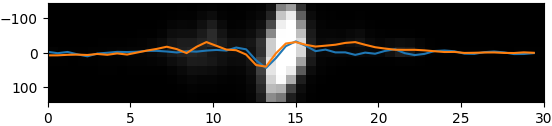
\includegraphics[width=\textwidth]{fig/doppler_1182}
					\end{subfigure}
					~ 
					\begin{subfigure}[t]{0.49\textwidth}
						\centering
						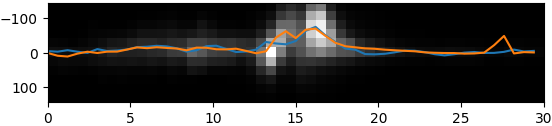
\includegraphics[width=\textwidth]{fig/doppler_1225}
					\end{subfigure}
					~ 
					\begin{subfigure}[t]{0.49\textwidth}
						\centering
						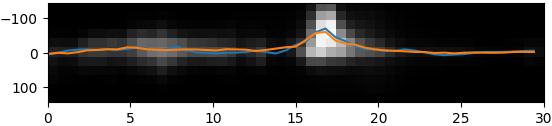
\includegraphics[width=\textwidth]{fig/doppler_1263}
					\end{subfigure}
					~ 
					\begin{subfigure}[t]{0.49\textwidth}
						\centering
						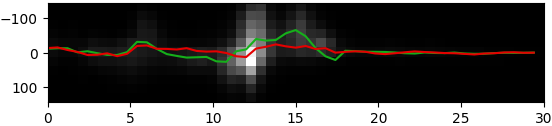
\includegraphics[width=\textwidth]{fig/doppler_1343}
					\end{subfigure}
					\caption{Examples of Doppler inversions. Each image is an IRIS \SiIV\ spectra rebinned into \MOSES\ resolution. The vertical axis is in km/s and the horizontal axis is in arcsec. The true line center is plotted in orange, and the reconstructed line center is plotted in blue.}
					\label{dopp_ex}
				\end{figure*}

				In Figure \ref{din_hist} we constructed a histogram of the true velocity vs. the reconstructed velocity for every pixel in our validation dataset to demonstrate the statistical effectiveness of our method.
				If the DIN reconstruction were perfect, the result of this plot would be a straight line with slope unity (plotted in blue).
				Immediately, we can see that the reconstruction is not flawless. 
				There is an obvious spread about the line of perfect reconstruction, biased towards slower speeds.
				
				For comparison with Figure \ref{din_hist} we have provided an analogous image (Figure \ref{smart_hist}) prepared using the \SMART, the de-facto standard algorithm for inverting MOSES observations.
				This image is a scatterplot constructed from a single SUMER O\,\textsc{iii} 703.87 \AA\ raster.
				Since Figure \ref{smart_hist} is only constructed from a single raster, it contains much less samples than Figure \ref{din_hist}, and therefore the two should not be compared directly.
				However, SMART's underestimation of velocity is a well-studied phenomenon, so we know that Figure \ref{smart_hist} reasonably demonstrates SMART's capabilities.
				
				With the above considerations we can see that according to Figure \ref{dopp_hist} the \DIN\ is much less likely to underestimate the velocity than this implementation of SMART.
				However these results are still preliminary and obviously need to be verified by applying SMART to the same IRIS dataset used to validate the DIN.
				
				A quantitative test that we preformed on Figure \ref{din_hist} was the calculation of Pearson's $r$, a test of linearity.
				The result, enumerated in Table \ref{nn_table} as $r = 0.701$, we interpret as modest performance, likely polluted by spikes in the input dataset.
			
				\begin{figure*}[h!]
					\centering
					\begin{subfigure}[t]{0.5\textwidth}
						\centering
						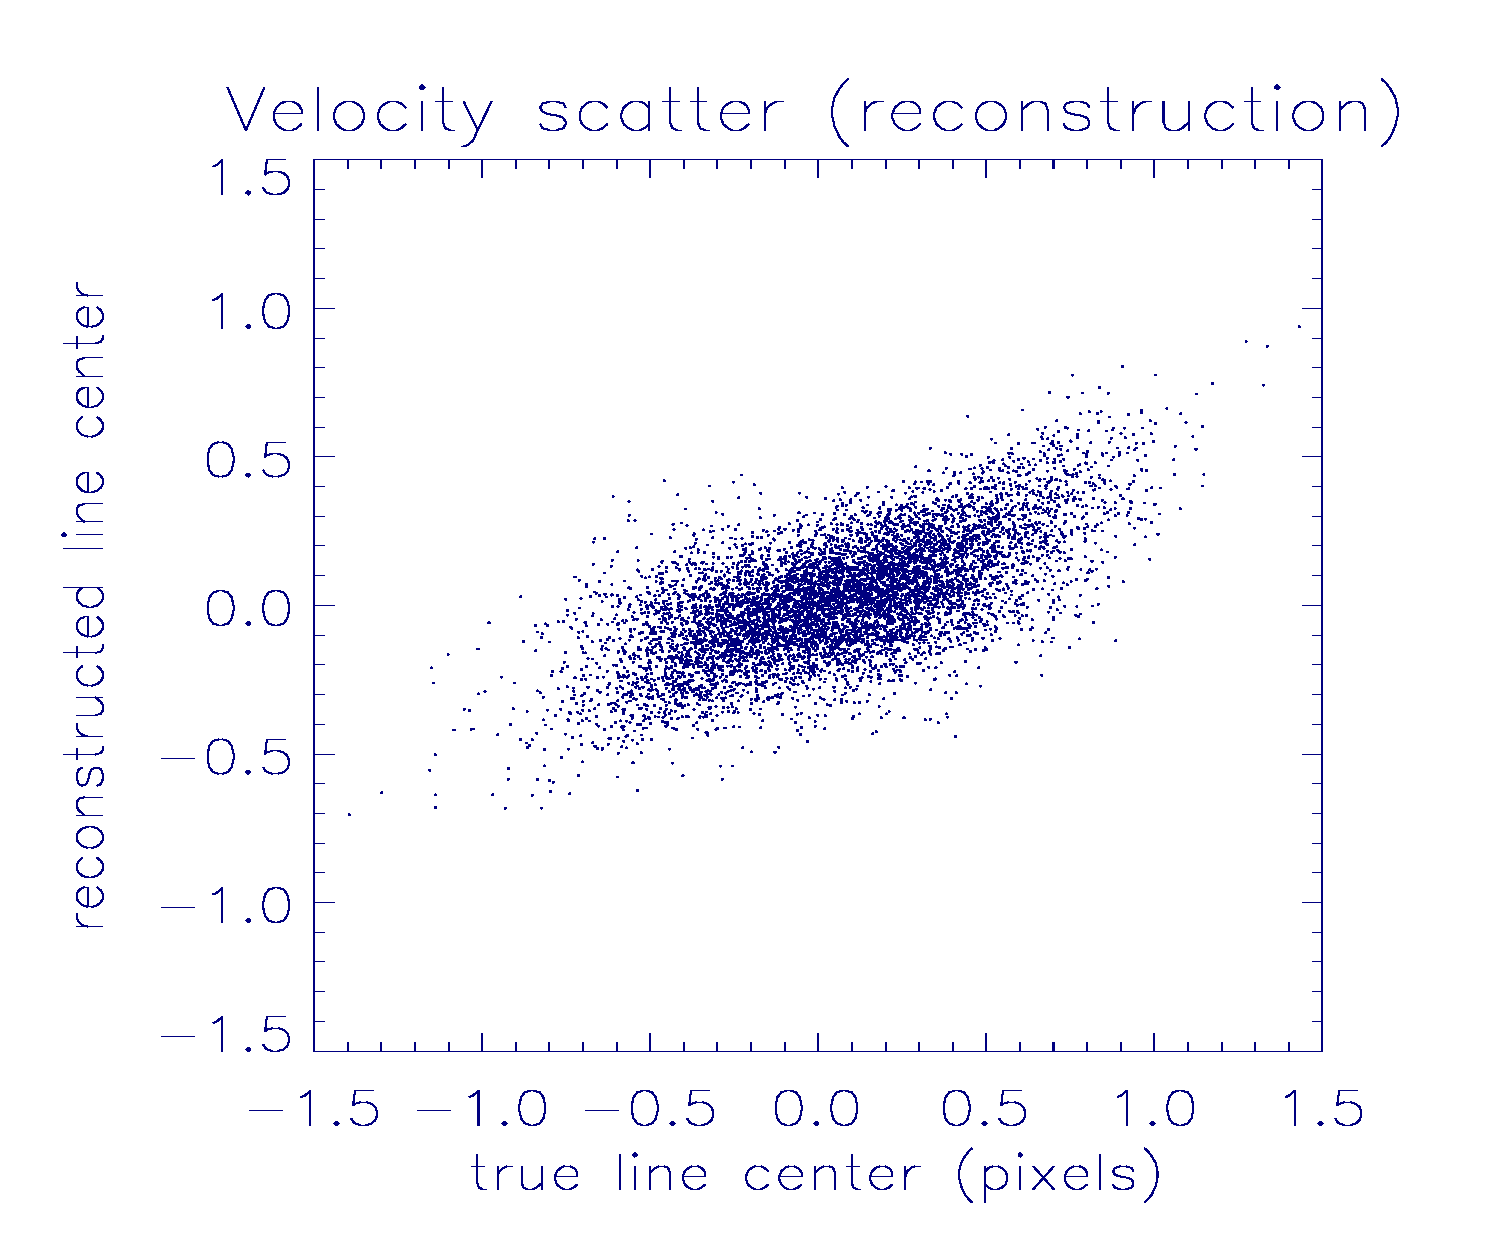
\includegraphics[width=\textwidth]{fig/smart_hist}
						\caption{SMART}
						\label{smart_hist}
					\end{subfigure}%
					~ 
					\begin{subfigure}[t]{0.5\textwidth}
						\centering
						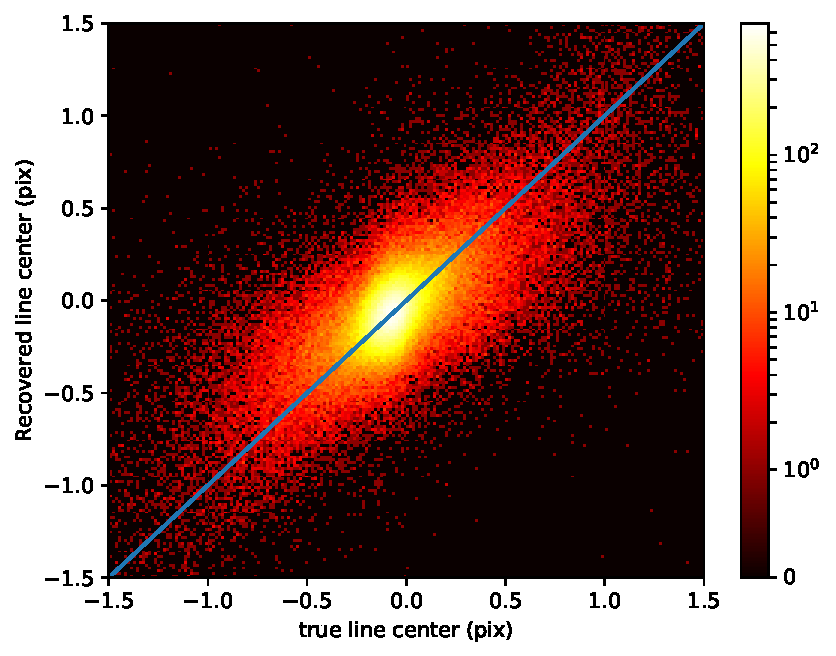
\includegraphics[width=\textwidth]{fig/linearity}
						\caption{DIN}
						\label{din_hist}
					\end{subfigure}
					\caption{Reconstructed vs. true Doppler velocity using both the standard \SMART\ algorithm (applied to SUMER O\,\textsc{iii} 703.87 \AA\ raster; courtesy of Charles Kankelborg), and the CINN algorithm (applied to IRIS Si\,\textsc{iv} 1403 \AA.)}
					\label{dopp_hist}
				\end{figure*}
				
				
							
			\subsubsection{Despiking Training Data}	\label{sec_dspk}
			
				Spikes in IRIS observations are a stochastic process, primarily due to ionospheric particles impacting the CCD detectors.
				Removal of spikes in our training dataset is important since the network will become distracted trying to reconstruct the spikes, a futile undertaking.
				This was not considered to be a serious problem during the proposal phase, as there have been several despiking routines written for IRIS.
				However we failed to appreciate how difficult it would be to apply these routines in an automated fashion to a large section of the IRIS \SiIV\ dataset.
				
				There are a multitude of despiking routines available on the IDL SolarSoft libraries, such as \texttt{nospike.pro}, \texttt{array\_despike.pro}, \texttt{iris\_prep\_despike.pro}.
				Unfortunately they all identify spikes using the same method: convolution of some kernel with an image to estimate a local mean and standard deviation, and a hard threshold to exclude pixels some number of standard deviations above the mean.
				This method is often too aggressive in areas of high signal intensity and not aggressive enough in areas of low signal intensity.
				In Figure \ref{dspk_ex}, we can see an example of this behavior: the explosive event in the bottom row has become eroded from \texttt{iris\_prep\_despike.pro}, while many of the spikes in the top row are only partially identified.
				Considering this behavior, to use these procedures we found that we would have to manually tune them for each observation, which would become prohibitive for a training dataset composed of many IRIS observations.
				
				Instead of estimating the mean and standard deviation, our method uses a median-percentile based approach, where pixels are marked as spikes if their value is larger than 99\% (for example) of all other pixels with the same median. 
				This is accomplished by calculating a local median for every pixel in the observation, and then constructing a histogram of median vs. pixel value for each observation.
				From this histogram, we can then determine the bad pixel threshold as a function of the local median.
				Finally, this procedure was performed independently along each axis (wavelength, space, time) and we required that a pixel must be above the threshold for all three axes to be marked as a spike.
				A visualization of this procedure is presented in Figure \ref{dspk_hist}, where we can see the threshold used to perform the despiking seen in Figure \ref{dspk_ex}.		
				We have developed a GPU implementation of this despiking procedure, resulting in code that is at least 10x faster than current methods while being much more discriminatory.
				
			
				\begin{figure}[h!]
					
					\centering
					\renewcommand{\arraystretch}{0}
					\setlength{\tabcolsep}{0pt}
					\begin{tabular}{m{0.1\textwidth} m{0.3\textwidth} m{0.3\textwidth} m{0.3\textwidth} @{}m{0pt}@{}}
						& \centering Original & \centering \texttt{iris\_prep\_despike.pro} & \centering Our Method & \\[5mm]
						Region 1 & 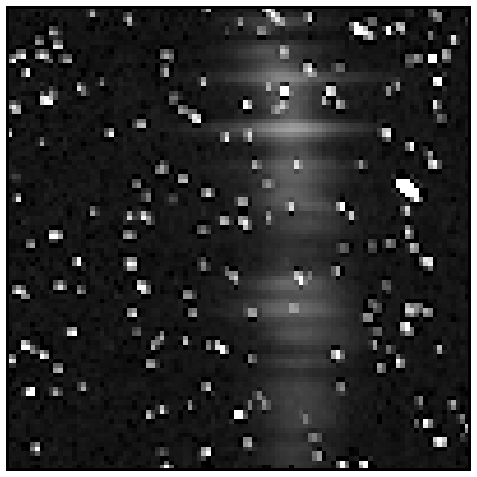
\includegraphics[width=0.3\textwidth]{fig/orig_1} & 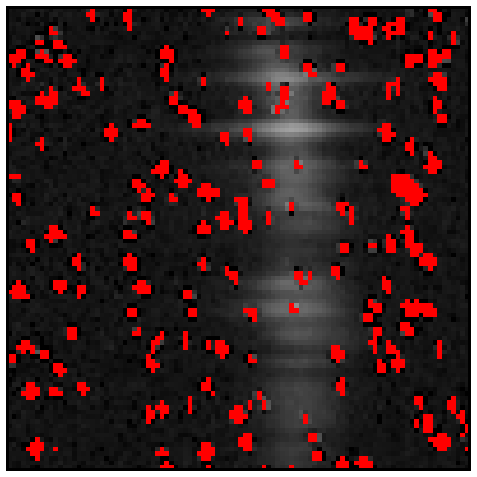
\includegraphics[width=0.3\textwidth]{fig/despike_1} & 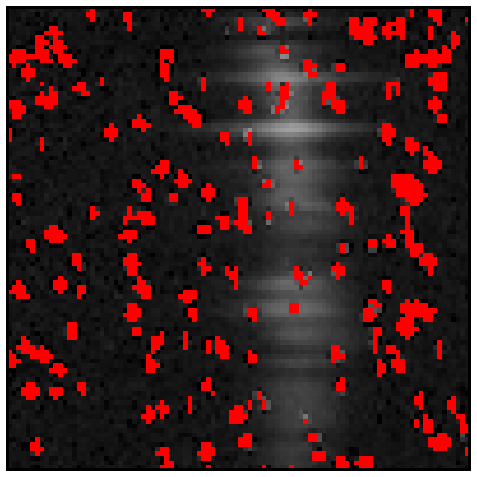
\includegraphics[width=0.3\textwidth]{fig/dspk_1} & \\
						Region 2 & 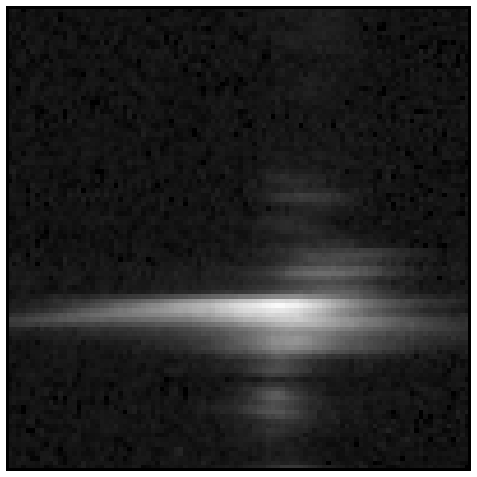
\includegraphics[width=0.3\textwidth]{fig/orig_2} & 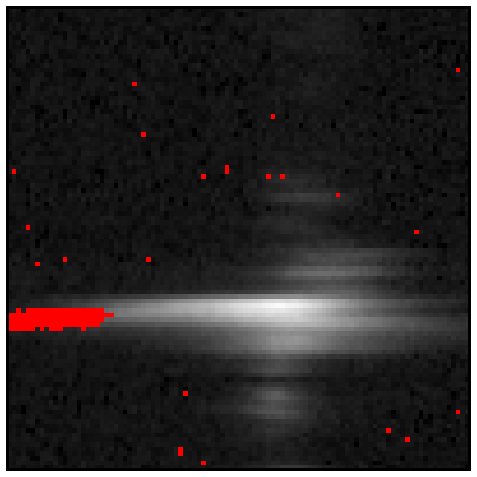
\includegraphics[width=0.3\textwidth]{fig/despike_2} & 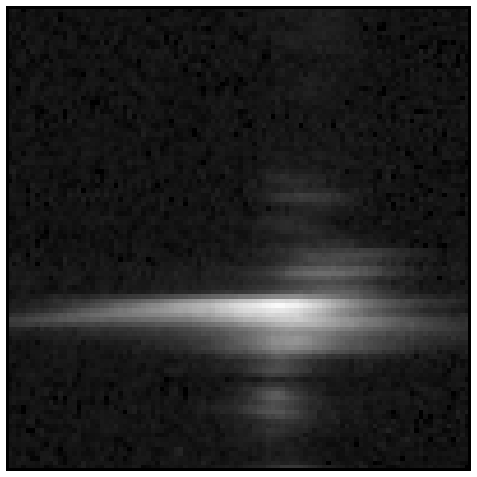
\includegraphics[width=0.3\textwidth]{fig/dspk_2} & \\
					\end{tabular}
					
					\caption{An example of both the standard despiking algorithm and our spike identification algorithm applied to an IRIS \SiIV\ observation gathered at 07:24:26 on 06-16-2015.
						Pixels containing spikes are marked red by each algorithm.
						We present cutouts from frames 24 and 50 to demonstrate how susceptible each algorithm is to false spike identifications. 
						The frame on the top row was taken inside the \SAA, and provides examples of many types of spikes intended to show the false negatives identified by each algorithm.
						The frame on the bottom row is an example of an \EE, and serves as an example of the false positives identified by each algorithm.}
					
					\label{dspk_ex}
					
				\end{figure}
				
				\begin{figure*}[h!]
					\centering
					\begin{subfigure}[t]{0.288\textwidth}
						\centering
						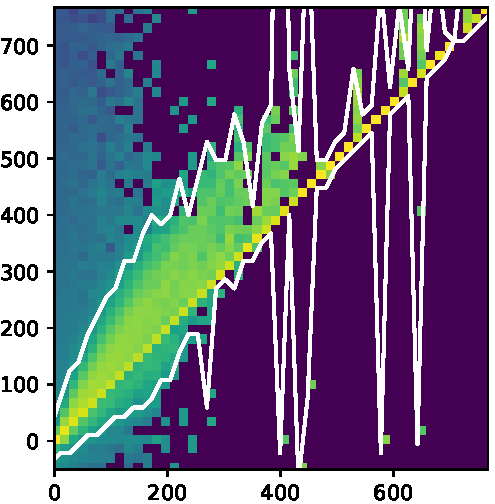
\includegraphics[width=\textwidth]{fig/hist_0}
						\caption{Wavelength}
					\end{subfigure}
					~ 
					\begin{subfigure}[t]{0.288\textwidth}
						\centering
						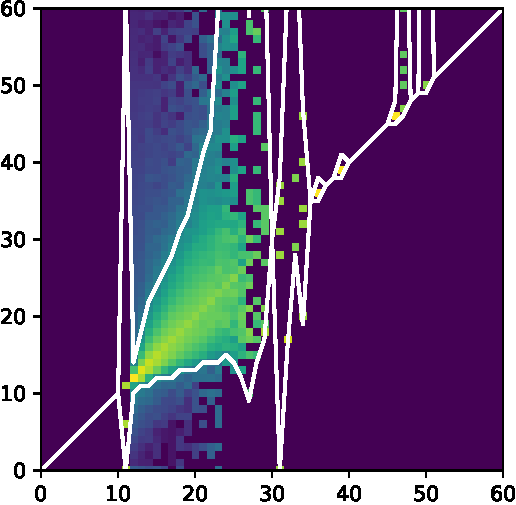
\includegraphics[width=\textwidth]{fig/hist_1}
						\caption{Space}
					\end{subfigure}
					~ 
					\begin{subfigure}[t]{0.288\textwidth}
						\centering
						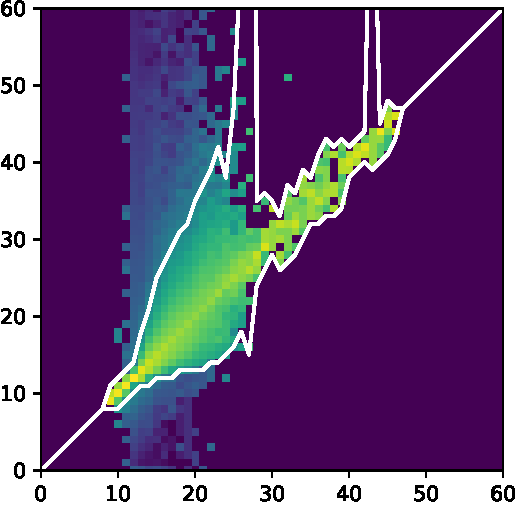
\includegraphics[width=\textwidth]{fig/hist_2}
						\caption{Time}
					\end{subfigure}
					~ 
					\begin{subfigure}[t]{0.079\textwidth}
						\centering
						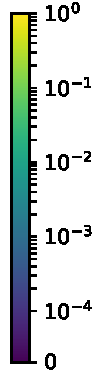
\includegraphics[width=\textwidth]{fig/cbar}
					\end{subfigure}
					
					\caption{Column-normalized histogram along each axis for the observation in Figure \ref{dspk_ex}.
						Each column has been divided by its total to understand the distribution of values about a particular median.
						The 1\% and 99\% thresholds have been plotted in white.
						Horizontal and vertical axes are in DN.}
					
					\label{dspk_hist}
					
				\end{figure*}
		
		\subsection{FURST Design}
	
	\section{Proposal for Renewal}
	
		\subsection{MOSES Inversion GAN} \label{sec_gan}
		
		
		\subsection{Explosive Event Classification}
		

	
	\section{Conclusion}
	\begin{landscape}
		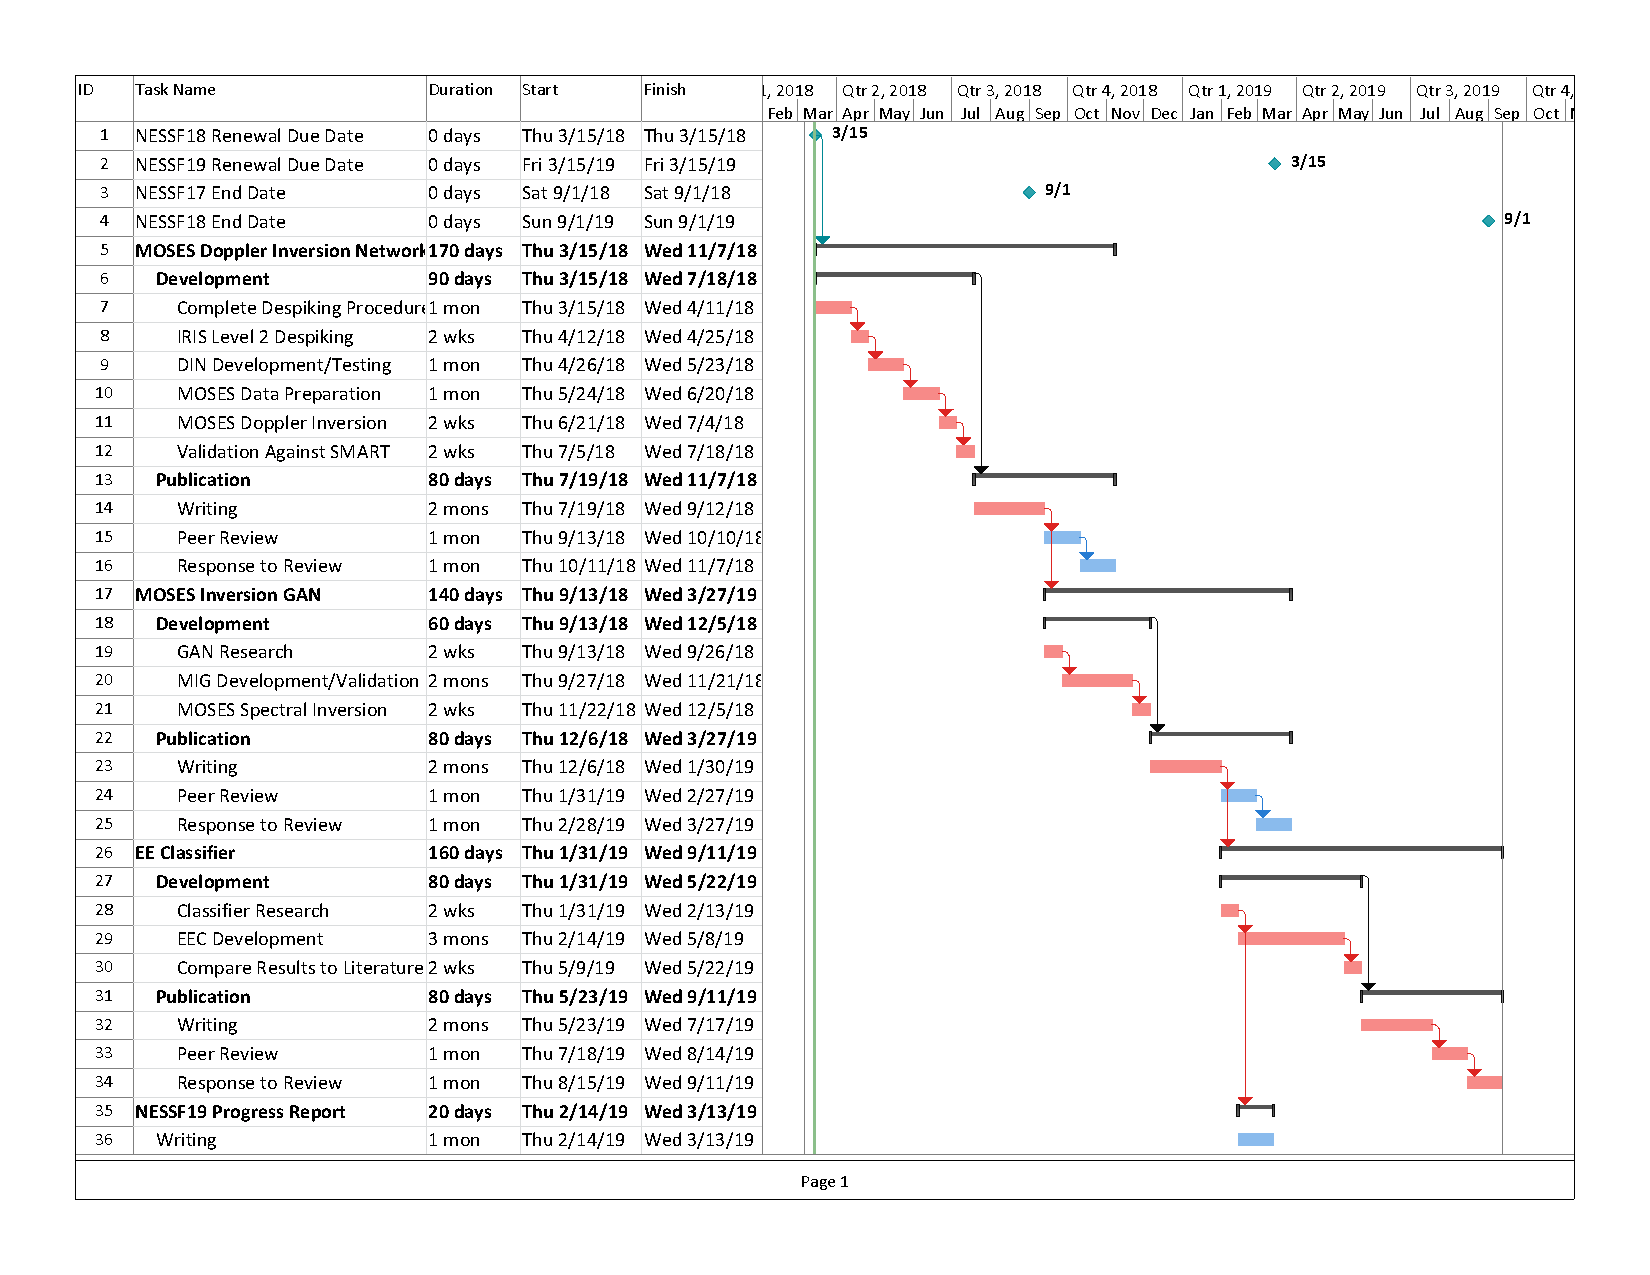
\includepdf[pages=-,landscape=true]{../schedule/NESSF18_schedule}
%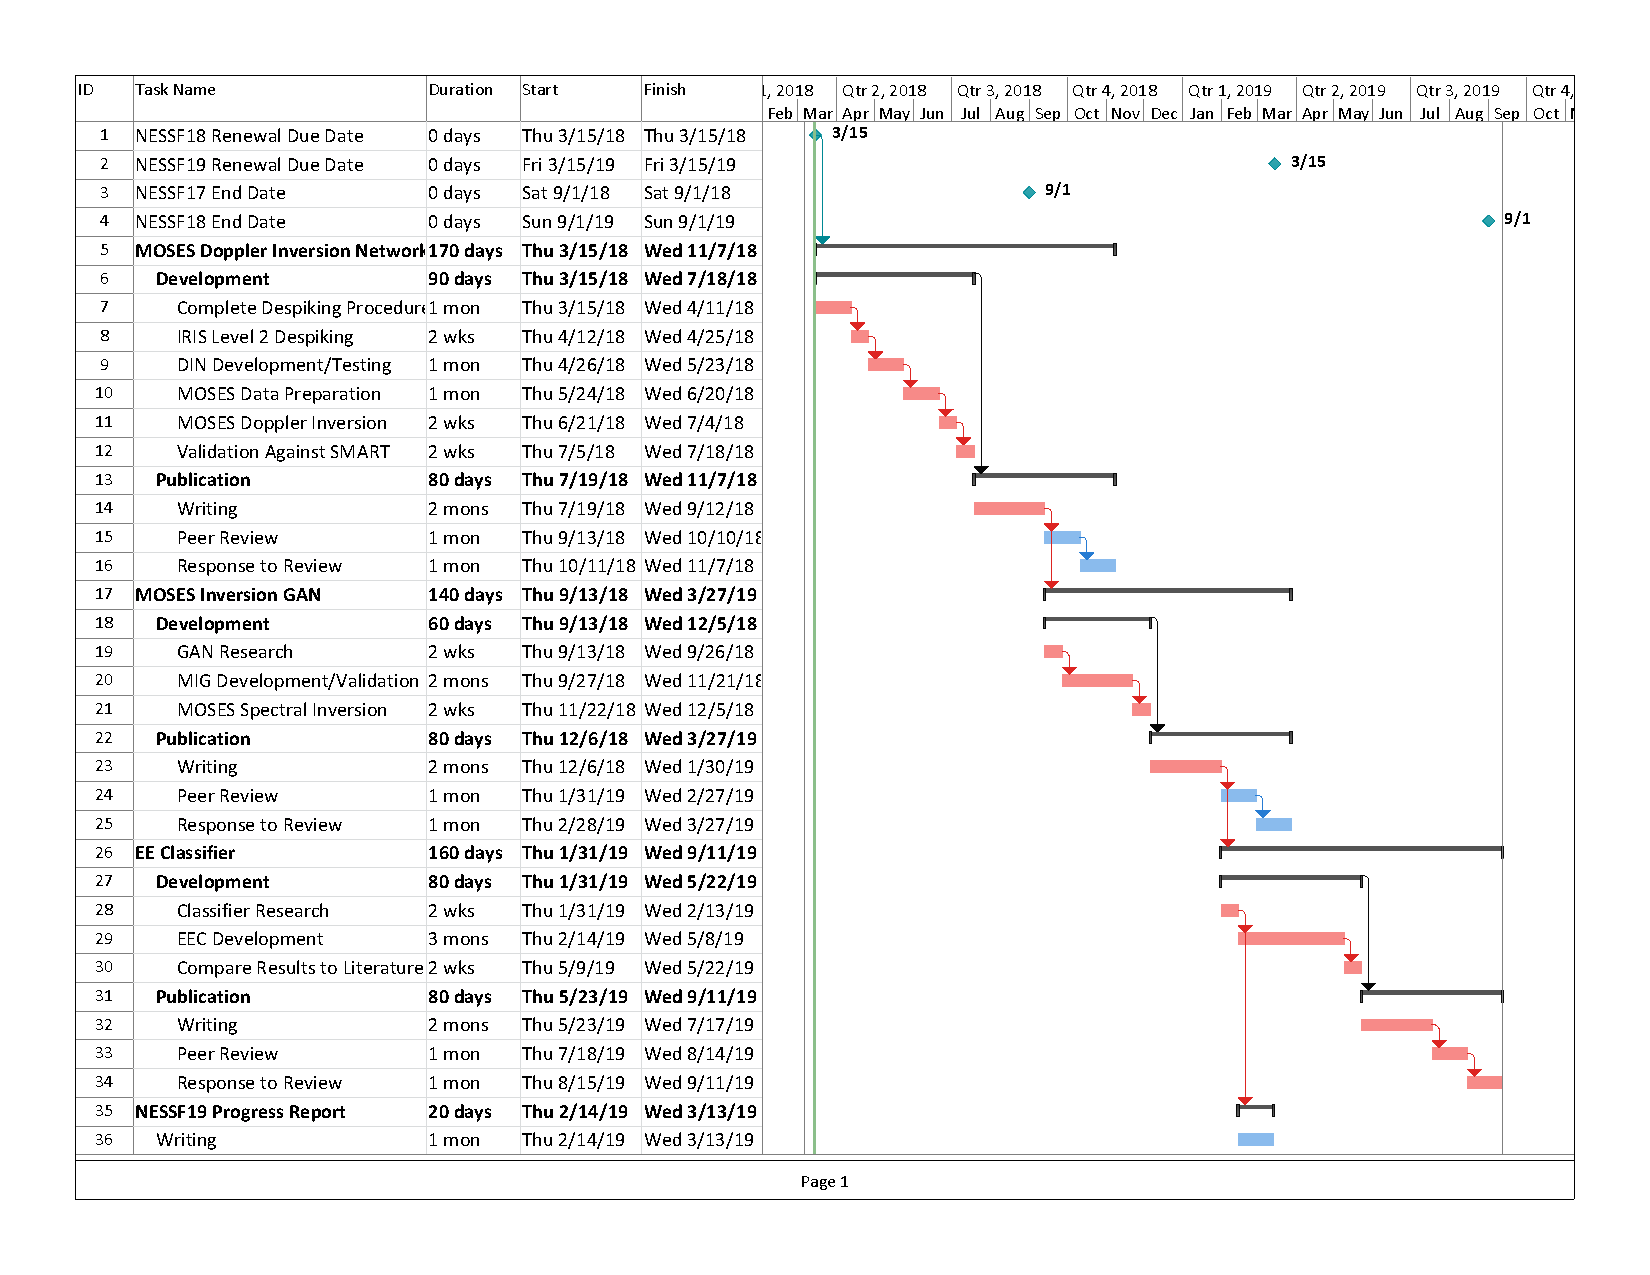
\includegraphics[width=\textwidth]{../schedule/NESSF18_schedule}
	\end{landscape}
	
\end{document}